\documentclass[10pt,a4paper]{article}

\usepackage[utf8]{inputenc}
\usepackage[T1]{fontenc}
\usepackage[spanish,es-noshorthands,es-tabla]{babel}
\usepackage[top=1.6cm,bottom=1.6cm,left=1.8cm,right=1.8cm]{geometry}
\usepackage{graphicx}
\usepackage{booktabs}
\usepackage{array}
\usepackage{multirow}
\usepackage{xcolor}
\usepackage{caption}
\usepackage{listings}
\usepackage{enumitem}
\usepackage{titlesec}
\usepackage{needspace}
\usepackage{multicol}
\usepackage{tocloft}
\usepackage[colorlinks=true,linkcolor=blue!50!black,urlcolor=blue!50!black]{hyperref}

% ---- compacidad ----
\setcounter{tocdepth}{1}
\renewcommand{\cftsecfont}{\small}
\renewcommand{\cftsecpagefont}{\small}
\setlength{\cftbeforesecskip}{0pt}
\renewcommand{\cftdotsep}{2}
\setlength{\parskip}{0.3em}
\setlength{\tabcolsep}{3pt}
\setlength{\emergencystretch}{3em}
\setlength{\parindent}{0pt}
\setlist{nosep,leftmargin=1.3em}
\titlespacing*{\section}{0pt}{0.9em}{0.35em}
\titlespacing*{\subsection}{0pt}{0.6em}{0.25em}
\titleformat{\section}{\large\bfseries}{\thesection.}{0.5em}{}
\titleformat{\subsection}{\normalsize\bfseries}{\thesubsection}{0.5em}{}
\captionsetup{font=small,labelfont=bf,skip=3pt}
\setlength{\textfloatsep}{8pt plus 2pt minus 2pt}
\setlength{\floatsep}{6pt plus 2pt minus 2pt}
\setlength{\intextsep}{6pt plus 2pt minus 2pt}
\renewcommand{\topfraction}{0.95}
\renewcommand{\bottomfraction}{0.95}
\renewcommand{\textfraction}{0.05}
\renewcommand{\floatpagefraction}{0.8}
\renewcommand{\arraystretch}{1.05}

\definecolor{ok}{HTML}{16A34A}
\definecolor{pend}{HTML}{6B7280}
\newcommand{\hecho}{\textcolor{ok}{\textbf{Hecho}}}
\newcommand{\pend}{\textcolor{pend}{Pendiente}}
\newcommand{\ruta}[1]{\texttt{\footnotesize #1}}
% diagrama de StarUML recortado: \stfig{archivo}{trim: izq abajo der arriba}{ancho}
\newcommand{\stfig}[3]{\includegraphics[width=#3,trim=#2,clip]{staruml/#1.pdf}}

\lstset{
  basicstyle=\ttfamily\scriptsize, showstringspaces=false, frame=single, rulecolor=\color{gray!50},
  breaklines=true, columns=fullflexible, numbers=left, numberstyle=\tiny\color{gray}, xleftmargin=1.6em,
  aboveskip=2pt, belowskip=2pt,
  literate={á}{{\'a}}1 {é}{{\'e}}1 {í}{{\'i}}1 {ó}{{\'o}}1 {ú}{{\'u}}1 {ñ}{{\~n}}1
           {Á}{{\'A}}1 {É}{{\'E}}1 {Í}{{\'I}}1 {Ó}{{\'O}}1 {Ú}{{\'U}}1 {Ñ}{{\~N}}1
           {¿}{{?`}}1 {¡}{{!`}}1 {—}{{---}}1 {→}{{->}}1 {≤}{{<=}}1 {±}{{+/-}}1 {°}{{$^\circ$}}1
           {“}{{"}}1 {”}{{"}}1 {…}{{...}}1 {·}{{.}}1
}

\begin{document}

\begin{center}
{\LARGE\bfseries Civic Security}\\[2pt]
{\large Informe de avance del MVP --- backend, frontend y base de datos}\\[3pt]
{\small Curso ET201, Formación de Empresas de Base Tecnológica I --- Universidad Católica San Pablo\\
Integrantes: \textit{Anthony Briceño, Maycol Canaveri y Marcelo Torres} \quad|\quad 5 de noviembre de 2026}
\end{center}
\vspace{-0.3em}

{\small\textbf{Índice}}\vspace{-0.4em}
\begin{multicols}{2}
\makeatletter\@starttoc{toc}\makeatother
\end{multicols}
\vspace{-0.5em}

% ============================================================
\section{Resumen}
Civic Security es una red ciudadana para reportar incidentes de seguridad de forma anónima y validarlos de forma comunitaria en Arequipa. El MVP funciona hoy de punta a punta para \textbf{ver reportes en un mapa y enviar un reporte anónimo}; la \textbf{validación comunitaria}, diferencial del producto, está diseñada y queda para las siguientes iteraciones. Repositorio público: \url{https://github.com/aaabriceno/Proyecto-MVP-Civic-Security}.

\begin{itemize}
  \item \textbf{Funciona hoy:} mapa centrado en la ubicación del usuario con los reportes del servidor, filtros por tipo, detalle y envío de un reporte anónimo (tipo, ubicación, descripción).
  \item \textbf{Anonimato por diseño:} el reporte no tiene campo de usuario, no se guarda la IP con él y se rechazan datos personales (DNI, teléfonos, correos, enlaces) en la descripción.
  \item \textbf{Calidad y seguridad:} 61 pruebas del backend y 120 de la app en verde; análisis estático y auditoría de dependencias sin hallazgos; revisión con ataques reales al servidor y 12 hallazgos corregidos.
\end{itemize}

\begin{center}\footnotesize
\begin{tabular}{@{}lllr@{}}
\toprule
\textbf{Indicador (5/11/2026)} & \textbf{Código} & \textbf{Pruebas} & \textbf{Commits}\\
\midrule
Backend (Elixir/Phoenix) & 897 líneas, 23 archivos & 61 pruebas, 810 líneas & \multirow{2}{*}{19}\\
App (Flutter) & 2\,438 líneas, 24 archivos & 120 pruebas, 2\,138 líneas & \\
\bottomrule
\end{tabular}
\end{center}

% ============================================================
\section{Estado del MVP frente al alcance}
{\footnotesize
\begin{tabular}{@{}p{6.9cm}p{1.3cm}p{8.5cm}@{}}
\toprule
\textbf{Funcionalidad} & \textbf{Estado} & \textbf{Nota}\\
\midrule
Base de datos con PostGIS y datos de prueba & \hecho & Tabla \texttt{incidentes} con índice espacial\\
API para crear reportes y API del mapa & \hecho & \texttt{POST /v1/incidents}, \texttt{GET /v1/map/snapshot}\\
Canal en tiempo real en el backend & \hecho & La app todavía no lo escucha\\
Mapa con ubicación del usuario, pines por tipo, filtros y detalle & \hecho & Frame 05 de Figma (parcial)\\
Formulario de reporte anónimo con 6 tipos & \hecho & Frames 06, 06c y 07 de Figma\\
Seguridad básica de la API y de la app & \hecho & Sección~\ref{sec:seguridad}\\
Pines nuevos en tiempo real en la app & \pend & Backend listo; falta la app\\
Cuentas, inicio de sesión y verificación por DNI & \pend & Frames 01--04 y 10\\
\textbf{Validación comunitaria (3 confirmaciones a $<$ 1 km)} & \pend & \textbf{Prioridad n.º 1 del equipo}\\
Mapa de calor, alertas por zona y foto con rostros difuminados & \pend & Frames 05b, 09, 06a y 06b\\
\bottomrule
\end{tabular}}

% ============================================================
\section{Base de datos}
\label{sec:bd}
El motor es \textbf{PostgreSQL 17 con PostGIS 3.5} en un contenedor Docker (\ruta{infra/docker-compose.yml}) que solo acepta conexiones locales. PostGIS resuelve dentro de la base de datos, con índices, las consultas geográficas del producto: reportes del área visible, reportes a menos de 1~km (regla de votación) y el futuro mapa de calor. El diseño se documenta en tres niveles (conceptual, lógico y físico); \textbf{verde = implementado, gris = planificado}.

\begin{figure}[!htbp]
\centering
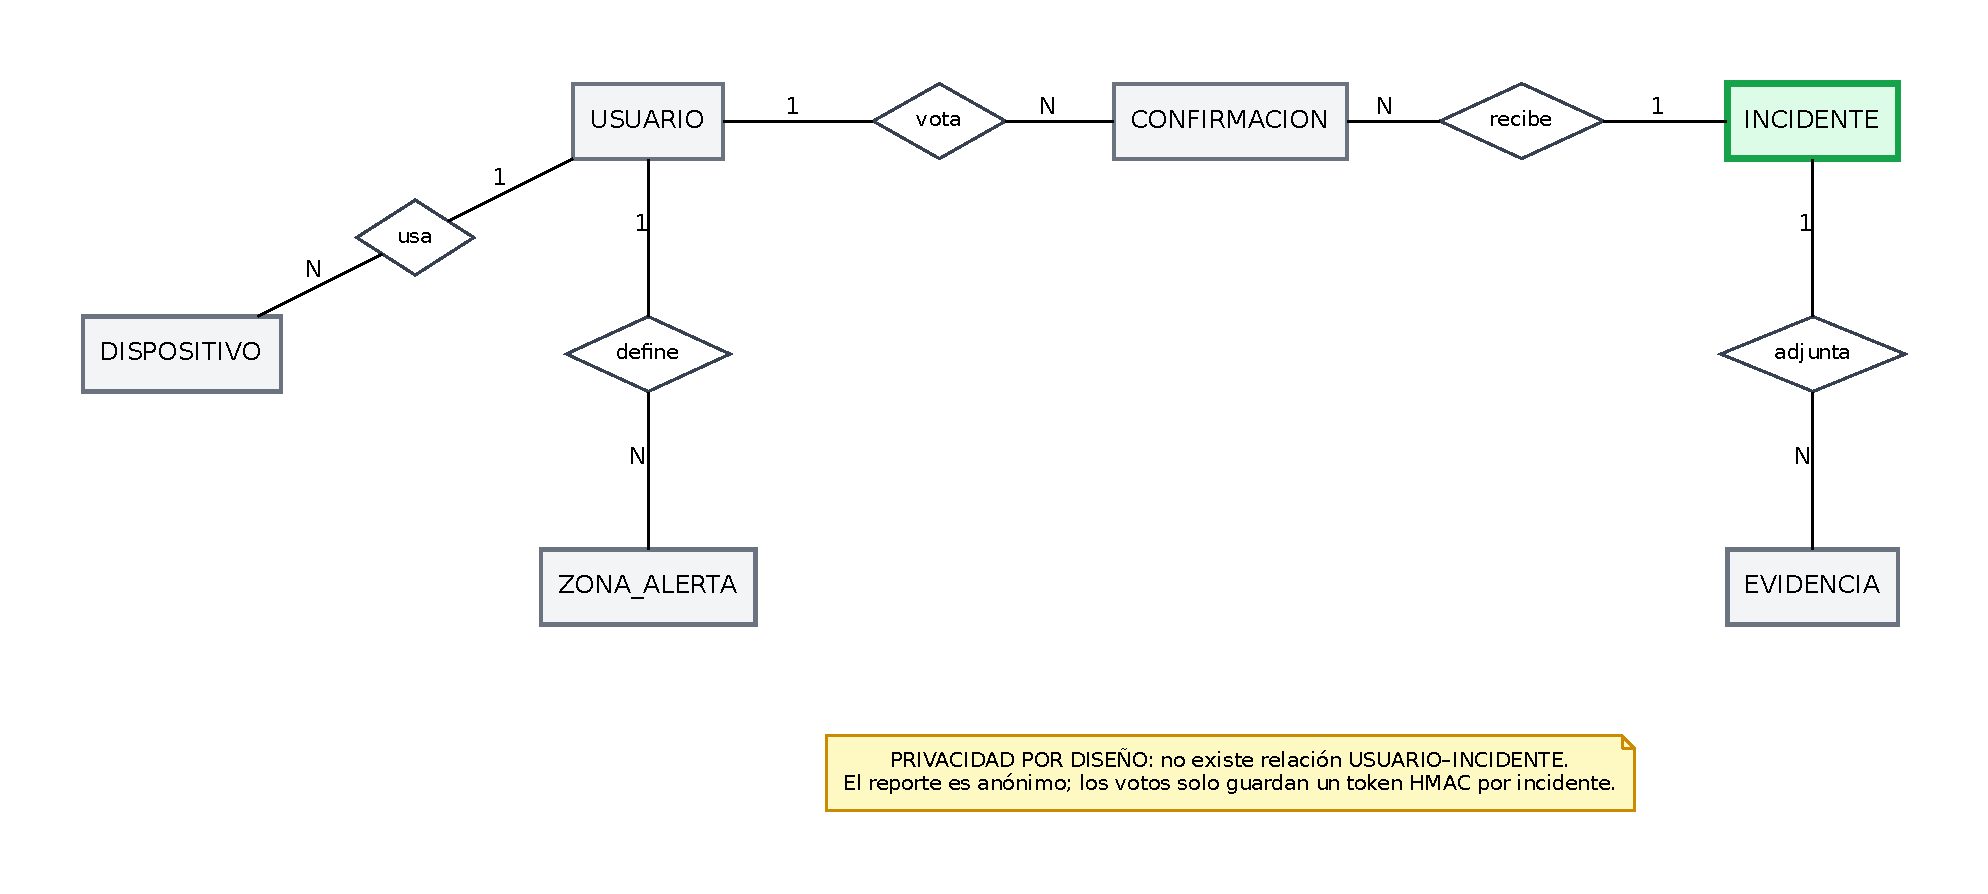
\includegraphics[width=0.95\textwidth]{diagramas/er-conceptual.pdf}
\caption{Modelo conceptual. Decisión de privacidad: \textbf{no existe relación entre USUARIO e INCIDENTE}.}
\end{figure}

\begin{figure}[!htbp]
\centering
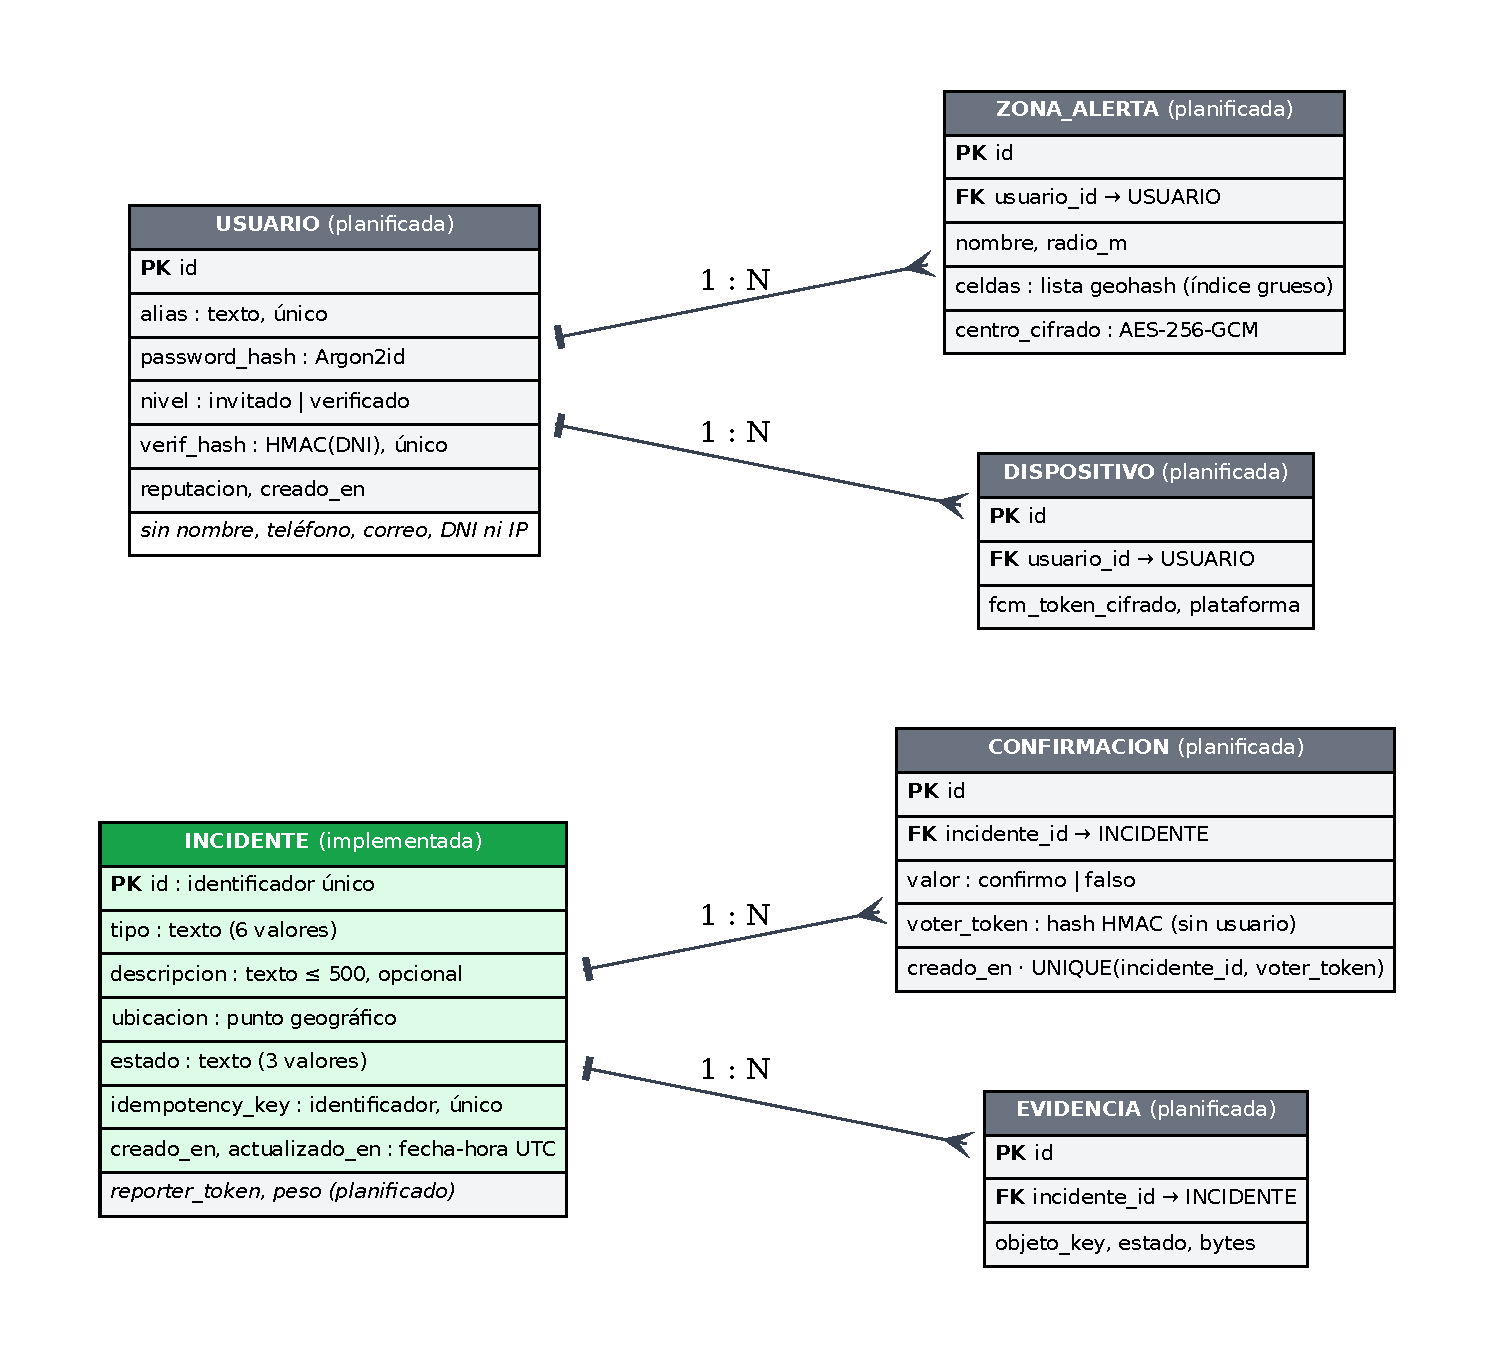
\includegraphics[width=0.8\textwidth]{diagramas/er-logico.pdf}
\caption{Modelo lógico: atributos, claves primarias (PK) y foráneas (FK).}
\end{figure}

\begin{figure}[!htbp]
\centering
\stfig{er-fisico}{61pt 24pt 37pt 69pt}{0.82\textwidth}
\caption{Modelo físico (StarUML): tipos de PostgreSQL. U = único, N = admite nulos. La tabla \texttt{incidentes} es la real (migración \ruta{20261027172454\_create\_incidentes.exs}).}
\end{figure}

\textbf{Decisiones de diseño:} identificadores \textbf{UUID} (los reportes no se pueden enumerar, OWASP API1:2023); \textbf{\texttt{geography(Point,}\allowbreak\texttt{4326)}} (distancias reales en metros; PostGIS guarda (longitud, latitud) y la API expone \texttt{lat} y \texttt{lng} por separado); índice \textbf{GiST} sobre \texttt{ubicacion} (las búsquedas por rectángulo del mapa no recorren todas las filas); \texttt{idempotency\_\allowbreak key} \textbf{único} (un reintento por mala señal no duplica el reporte); \textbf{ninguna columna identifica al usuario}; la verificación por DNI guardará solo un HMAC y no se guardan datos biométricos; el detalle se elimina a los 5 años.

Para la demostración hay 80 reportes \textbf{ficticios} (\ruta{backend/priv/repo/seeds.exs}), que pasan por las mismas reglas que la API, y consultas de ejemplo (\ruta{demo\_consultas.sql}): reportes por tipo y estado, filtros de tiempo, reportes a menos de 1~km (\texttt{ST\_DWithin}) y una agrupación en celdas de unos 500~m.

% ============================================================
\section{Backend}
Es un \textbf{monolito modular} en Elixir con Phoenix: el código se divide en módulos con responsabilidades claras (para mantenerlo) pero se despliega como un solo servicio con una sola base de datos (para operarlo y que rinda). La capa web (\ruta{lib/civic\_web}) solo recibe peticiones; las reglas viven en el dominio (\ruta{lib/civic}). Así, las reglas que distinguen al producto --- anonimato, área de Arequipa, no duplicados --- se aplican en el servidor y no en la app, que cualquiera puede modificar.

\begin{figure}[!htbp]
\centering
\stfig{componentes}{29pt 240pt 24pt 45pt}{0.97\textwidth}
\caption{Diagrama de componentes (StarUML). Verde: implementado; gris: planificado.}
\end{figure}

\subsection{API y reglas de negocio}
{\footnotesize
\begin{tabular}{@{}p{3.6cm}p{3.3cm}p{9.6cm}@{}}
\toprule
\textbf{Endpoint} & \textbf{Respuestas} & \textbf{Descripción}\\
\midrule
\texttt{GET /health} & 200, 429 & Comprueba que el servidor y la base de datos responden.\\
\texttt{POST /v1/incidents} & 201, 200, 400, 409, 413, 415, 422, 429 & Crea un reporte anónimo con el encabezado \texttt{idempotency-key}. 200 si se repite el mismo envío; 409 si la clave llega con otro contenido.\\
\texttt{GET /v1/map/snapshot} & 200, 400, 429 & Reportes de las últimas 24 h dentro del rectángulo \texttt{bbox=minLng,minLat,maxLng,maxLat} (máx. 500).\\
\texttt{WS /socket} & --- & Tópico \texttt{mapa:arequipa}: emite \texttt{incidente\_nuevo}; los clientes solo escuchan.\\
\bottomrule
\end{tabular}}

\begin{itemize}
  \item Seis tipos de incidente; todo reporte nace \textbf{``Sin verificar''} y el estado no se puede enviar desde el cliente (lista blanca de campos: \texttt{tipo}, \texttt{descripcion}, \texttt{lat}, \texttt{lng}).
  \item Ubicación obligatoria y dentro de Arequipa; descripción opcional de hasta 500 caracteres, sin caracteres de control ni datos personales; envío \textbf{idempotente}.
\end{itemize}

\begin{lstlisting}[caption={Cadena de validaciones (\ruta{backend/lib/civic/incidents/incident.ex}).}]
def create_changeset(incident, attrs) do
  incident
  |> cast(attrs, [:tipo, :descripcion, :lat, :lng])
  |> validate_required([:tipo, :lat, :lng])
  |> update_change(:descripcion, &trim_or_nil/1)
  |> validate_length(:descripcion, max: 500)
  |> validate_texto_seguro(:descripcion)
  |> validate_sin_datos_personales(:descripcion)
  |> validate_arequipa()
  |> put_ubicacion()
  |> unique_constraint(:idempotency_key)
end
\end{lstlisting}

\begin{figure}[!htbp]
\centering
\stfig{clases-backend}{35pt 24pt 137pt 41pt}{0.68\textwidth}
\caption{Diagrama de clases (módulos) del backend, con sus firmas reales (StarUML).}
\end{figure}

\subsection{Evidencia: respuestas reales de la API}
\begin{lstlisting}[numbers=none]
$ POST /v1/incidents (robo, lat -16.3963, lng -71.5340; el cliente intenta colar "estado":"verificado")
HTTP/1.1 201 Created   {"data":{"id":"a2392f57-...","estado":"sin_verificar","tipo":"robo", ...}}  <- se ignora
(mismo envio repetido con la misma clave) ......... HTTP 200
(sin encabezado idempotency-key) .................. HTTP 400 idempotency_key_required
(reporte en Lima) ................................. HTTP 422 "La ubicacion debe estar dentro de Arequipa"
(descripcion con un telefono) ..................... HTTP 422 "no escribas datos personales"
(cuerpo mayor a 8 KB) ............................. HTTP 413
\end{lstlisting}

% ============================================================
\section{Frontend (aplicación móvil Android)}
App en \textbf{Flutter (Dart)}, probada en Android. Usa \textbf{Riverpod} (estado), \textbf{flutter\_map} con OpenStreetMap (mapa), \textbf{geolocator} (ubicación) y \textbf{Dio} (API), organizada por funcionalidades (\textit{feature-first}): \texttt{core/} (límites de Arequipa, ubicación, red, marcador del 105) y \texttt{features/} (\texttt{incident}: modelo y repositorio; \texttt{map}: mapa, pines, filtros, lista, detalle; \texttt{report}: formulario, ajuste de ubicación y confirmación). Se siguen los mockups de Figma (frames 05, 06, 06c y 07). Las capturas se tomaron en un emulador Android contra el backend real, con datos ficticios.

\begin{figure}[!htbp]
\centering
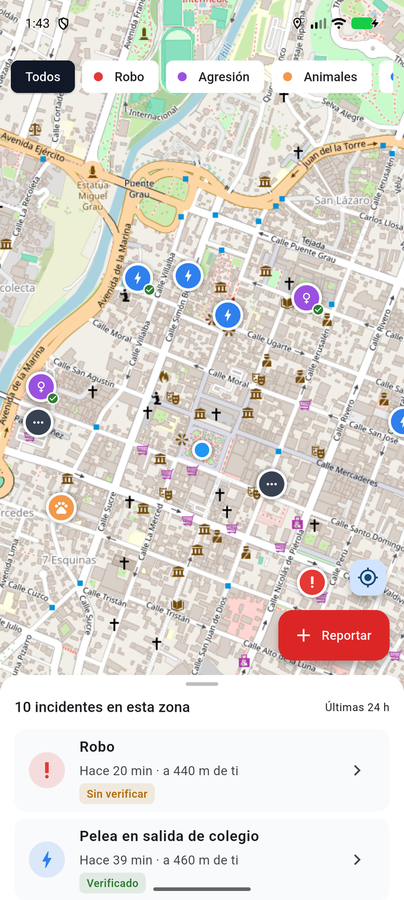
\includegraphics[height=6.1cm]{capturas/01-mapa.png}\hspace{3pt}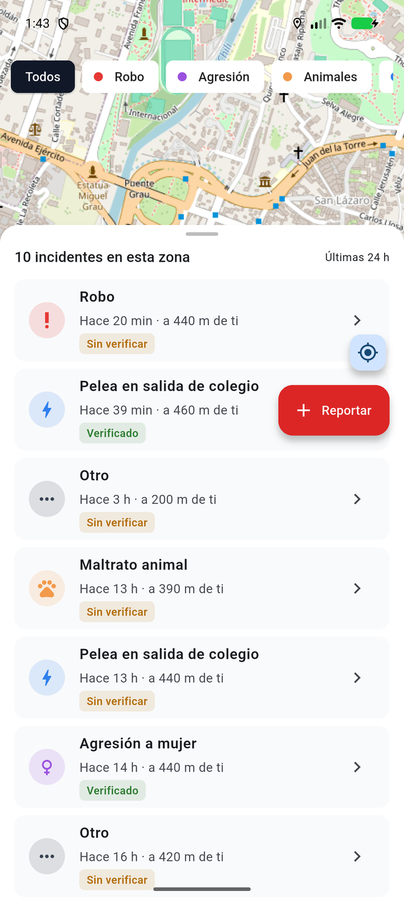
\includegraphics[height=6.1cm]{capturas/02-lista-expandida.png}\hspace{3pt}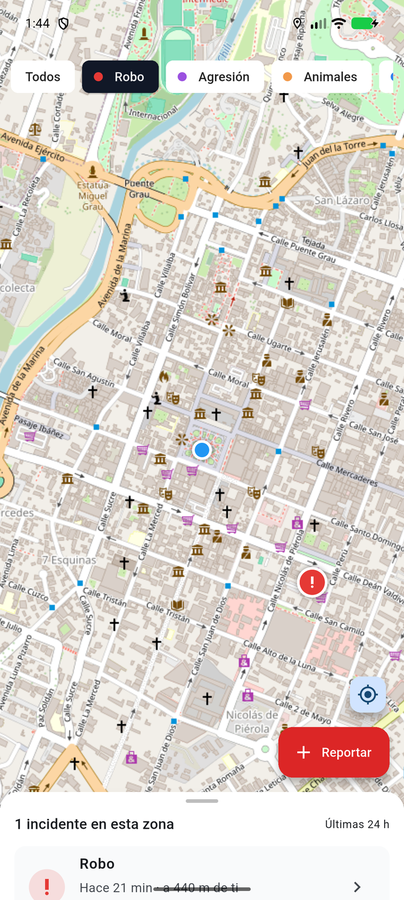
\includegraphics[height=6.1cm]{capturas/03-filtro-robo.png}\hspace{3pt}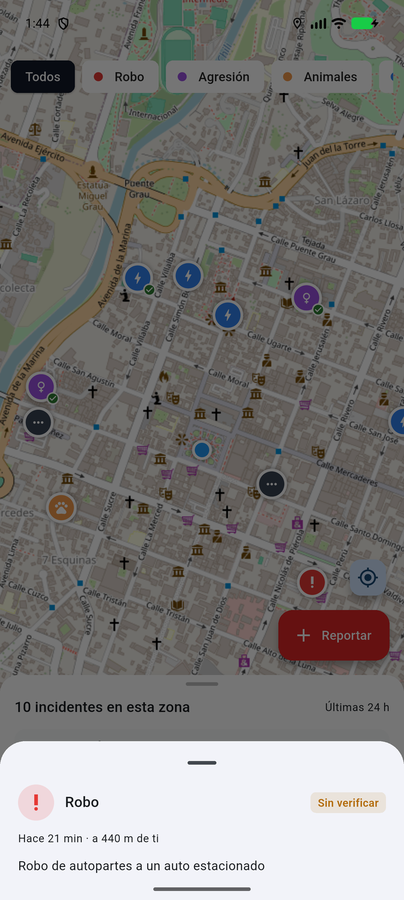
\includegraphics[height=6.1cm]{capturas/04-detalle.png}\\[3pt]
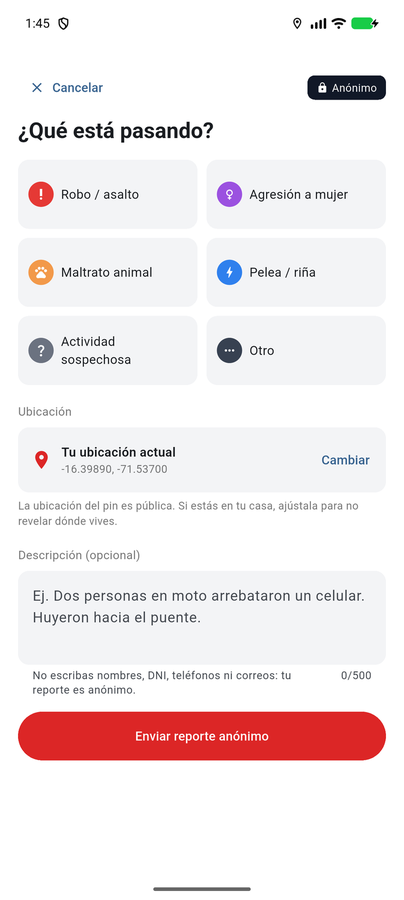
\includegraphics[height=6.1cm]{capturas/05-formulario.png}\hspace{3pt}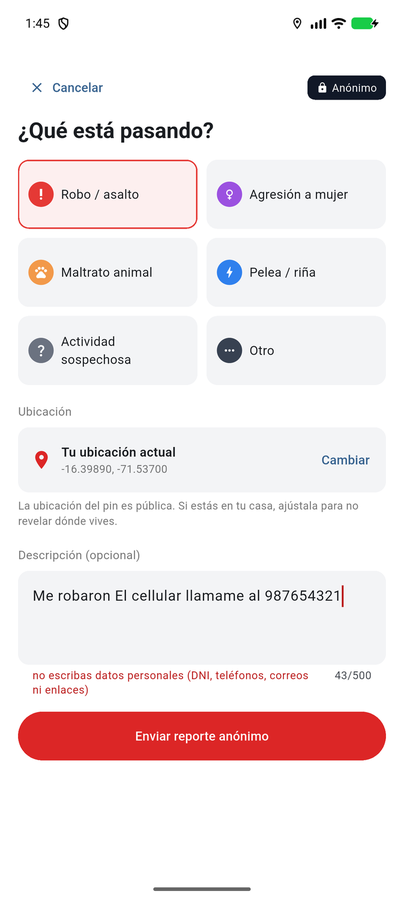
\includegraphics[height=6.1cm]{capturas/06-filtro-datos-personales.png}\hspace{3pt}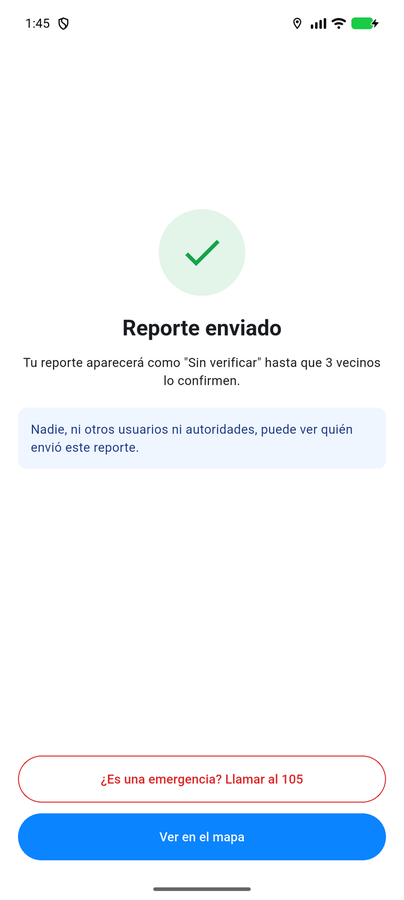
\includegraphics[height=6.1cm]{capturas/07-reporte-enviado.png}
\caption{Arriba: mapa con pines por tipo, lista ``N incidentes en esta zona'' con hora y distancia, filtro por tipo (Robo) y detalle. Abajo: formulario con los seis tipos; el servidor bloquea un teléfono escrito en la descripción y la app lo explica; confirmación con ``Llamar al 105''.}
\end{figure}

\textbf{Comportamientos relevantes:}
\begin{itemize}
  \item \textbf{Ubicación:} permiso en primer plano; el mapa se centra en el usuario. Sin permiso, con el GPS apagado o fuera de Arequipa, muestra Arequipa completa con un aviso; no inventa una ubicación.
  \item \textbf{Carga de datos:} pide solo los reportes del \emph{área visible}, tras 500~ms sin mover el mapa; una respuesta lenta no reemplaza a una más nueva y, ante un error de red, conserva los pines y ofrece ``Reintentar''.
  \item \textbf{Envío seguro ante mala señal:} cada formulario genera una clave de idempotencia; reintentar lo mismo no duplica. El botón se deshabilita mientras envía.
  \item \textbf{Privacidad y transporte:} la ubicación del usuario no sale del teléfono; en producción la app exige \texttt{https}.
\end{itemize}

\begin{figure}[!htbp]
\centering
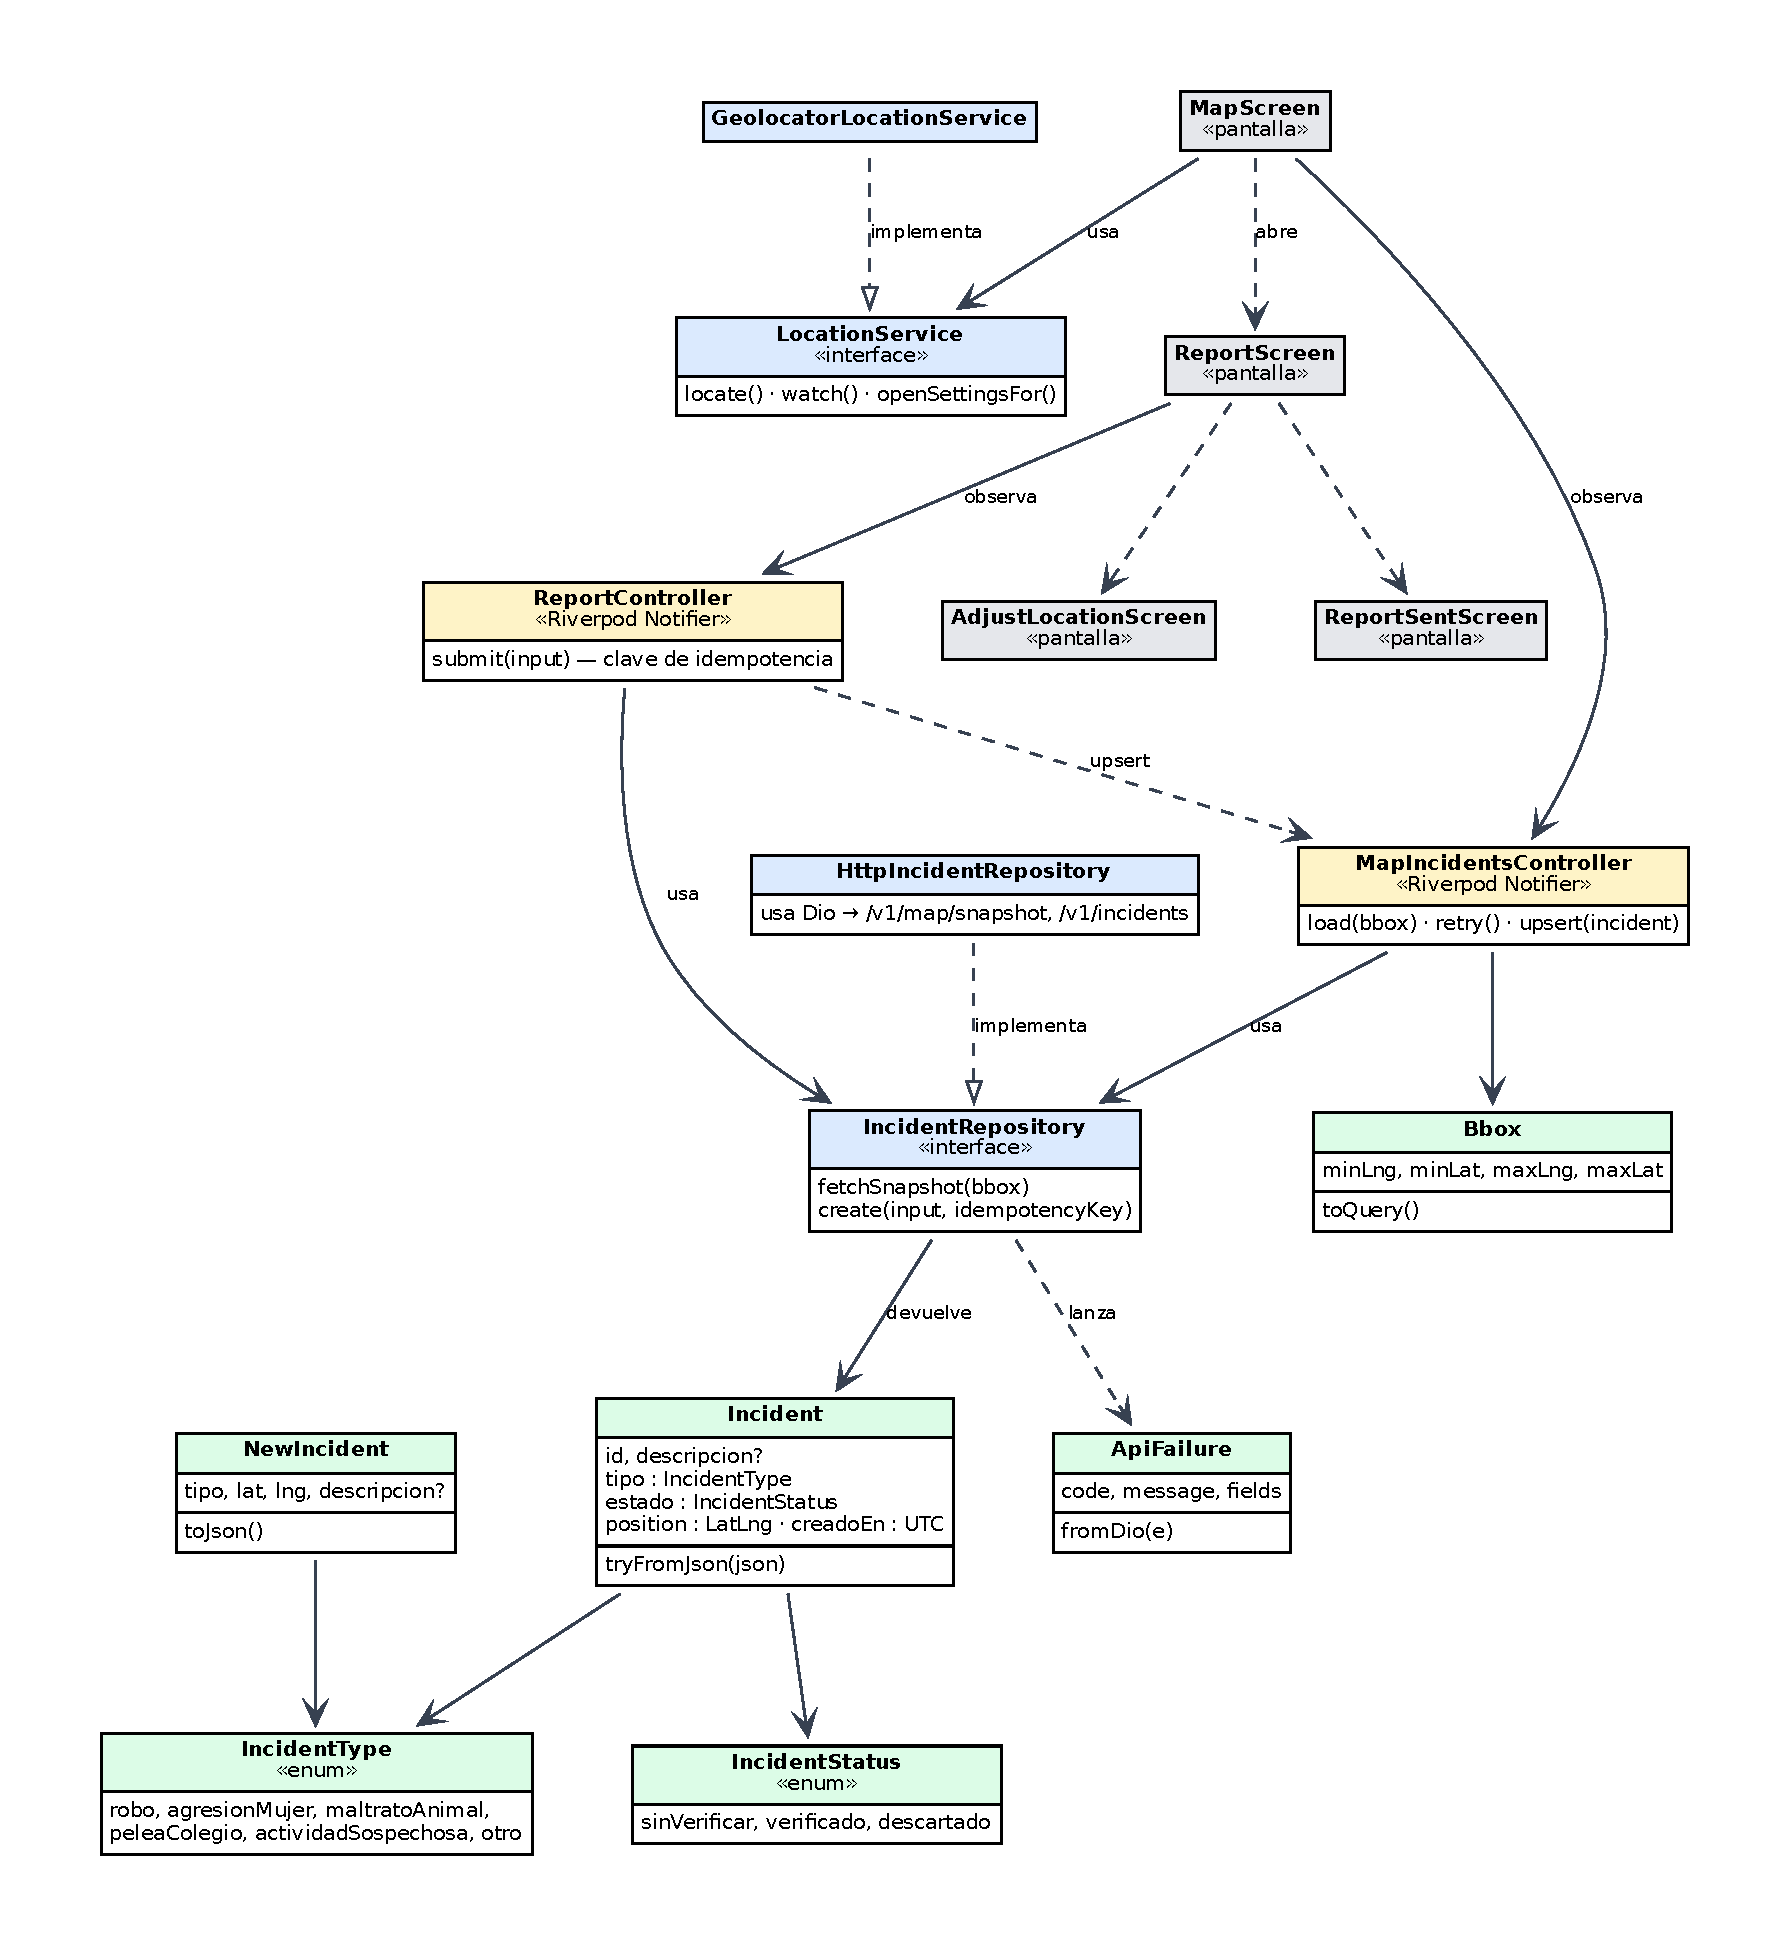
\includegraphics[width=0.78\textwidth]{diagramas/clases-app.pdf}
\caption{Diagrama de clases de la app: modelo, repositorio, controladores de estado y pantallas.}
\end{figure}

% ============================================================
\Needspace{16\baselineskip}
\section{Diagramas UML}
Elaborados con StarUML. \textbf{Verde = implementado; gris punteado = planificado.}

\begin{figure}[!htbp]
\centering
\stfig{casos-de-uso}{58pt 24pt 200pt 38pt}{0.62\textwidth}
\caption{Casos de uso del MVP. El usuario verificado generaliza al invitado: puede, además, confirmar o desmentir reportes y suscribir zonas de alerta.}
\end{figure}

\begin{figure}[!htbp]
\centering
\stfig{estados-incidentes}{40pt 323pt 24pt 45pt}{0.95\textwidth}
\caption{Estados del incidente. La columna \texttt{estado} ya admite los tres valores; las transiciones dependen de la validación comunitaria (iteración 2).}
\end{figure}

\begin{figure}[!htbp]
\centering
\stfig{secuencia}{44pt 222pt 25pt 51pt}{0.95\textwidth}
\caption{Secuencia: enviar un reporte anónimo. Si el servidor responde 200 (repetición con la misma clave) no se emite ningún evento.}
\end{figure}

\begin{figure}[!htbp]
\centering
\stfig{despliegue}{45pt 295pt 24pt 52pt}{0.95\textwidth}
\caption{Despliegue del entorno de pruebas: la tablet se conecta por USB y \texttt{adb reverse} lleva su puerto 4000 al servidor de la laptop, que sigue cerrado a la red.}
\end{figure}

% ============================================================
\section{Pruebas y seguridad}
\label{sec:seguridad}
\begin{lstlisting}[numbers=none]
$ cd backend && mix test ........ 61 tests, 0 failures     $ mix sobelow ........ sin hallazgos
$ mix deps.audit ................ No vulnerabilities found.   $ cd app && flutter analyze ... No issues found!
$ flutter test .................. +120: All tests passed!
\end{lstlisting}
Se trabajó con \emph{pruebas primero}: cada funcionalidad se describe con una prueba que falla y luego se implementa. Además se hizo una revisión actuando como atacante contra el servidor real, antes y después de cada corrección (informe completo en \ruta{docs/seguridad-revision-1.md}).

{\footnotesize
\begin{tabular}{@{}p{2.4cm}p{7.2cm}p{6.9cm}@{}}
\toprule
\textbf{Pilar} & \textbf{Hallazgo} & \textbf{Corrección}\\
\midrule
Disponibilidad & Sin límite de solicitudes (150 reportes seguidos aceptados); cuerpos de 3 MB y formularios aceptados; marcos y conexiones WebSocket sin límite & Límites por cliente (429); solo JSON de hasta 8 KB (413, 415); marco máx. 4 KB y límite de conexiones\\
Integridad & La misma clave con otro contenido perdía el reporte en silencio; APK firmado con la clave de depuración & Responde 409; el release queda sin firmar si falta la clave propia\\
Confidencialidad & Servidor de desarrollo abierto a toda la red y a cualquier origen; sin cabeceras de seguridad & Escucha solo en localhost y verifica el origen; \texttt{nosniff}, CSP, \texttt{no-store}\\
\bottomrule
\end{tabular}}

\textbf{Riesgos pendientes:} la app usa el superusuario de la base de datos (solo desarrollo; antes del piloto se creará un rol limitado); no hay cuentas, así que cualquiera puede reportar (límites generosos por IP porque muchos alumnos comparten el wifi de la universidad); los reportes con ubicación simulada se tratarán con la validación comunitaria.

% ============================================================
\section{Hallazgos de la prueba en tablet}
El 5 de noviembre se instaló la app en una tablet Android por USB contra el backend de la laptop. Funcionó de punta a punta; se investigaron dos observaciones:
\begin{enumerate}
  \item \textbf{Lentitud al cargar y mover el mapa.} \emph{Causa probable:} la prueba se hizo en modo \textbf{depuración} de Flutter, entre 3 y 10 veces más lento que la app real, en un dispositivo de gama media. \emph{Descartado:} la descarga de teselas (\texttt{flutter\_map} las guarda en disco y cancela las innecesarias). \emph{Acción:} se habilitó el modo \textbf{profile} para medir con el backend local; si la medición lo justifica, se limitará y agrupará los pines dibujados y se simplificarán sombras, para que la app funcione con fluidez en dispositivos de distintas capacidades.
  \item \textbf{Distancia (``a 660 m de ti'') que parecía corta.} La fórmula de la app coincide con el cálculo exacto de PostGIS (\ruta{app/test/core/distance\_test.dart}: 3\,208~m Plaza de Armas--Alto Selva Alegre, 431~m a la UCSP). Es distancia en \textbf{línea recta}, no por calles, y puede diferir de lo que se aprecia si la \textbf{ubicación del dispositivo} es imprecisa (una tablet sin GPS ubica por Wi-Fi, con errores de cientos de metros). \emph{Acción:} mostrar en el mapa un círculo con la precisión de la ubicación.
\end{enumerate}

% ============================================================
\section{Plan para la próxima semana}
{\footnotesize
\begin{tabular}{@{}p{0.8cm}p{10.8cm}p{4.8cm}@{}}
\toprule
\textbf{Prio.} & \textbf{Actividad} & \textbf{Resultado esperado}\\
\midrule
1 & \textbf{Integración continua} (GitHub Actions): pruebas, análisis estático, auditoría de dependencias y búsqueda de secretos en cada cambio & Cada cambio queda con marca verde o roja\\
1 & \textbf{Tiempo real en la app}: escuchar \texttt{incidente\_nuevo} y reconectar pidiendo el snapshot & Un reporte aparece en otro teléfono sin recargar\\
1 & \textbf{Backend de cuentas}: sesión de invitado, registro con alias y contraseña (Argon2id), verificación por DNI con HMAC, límites por cuenta & Reportar y votar con cuenta\\
2 & \textbf{Pantallas de Figma} 01--04 (bienvenida, login, registro, recuperación) conectadas a las cuentas & Flujo de registro funcional\\
2 & \textbf{Rendimiento:} medir en modo \emph{profile} en la tablet y optimizar; círculo de precisión de la ubicación & Mapa fluido en distintos dispositivos\\
3 & \textbf{Validación comunitaria}: votos ``Lo confirmo'' / ``Es falso'', regla de 3 confirmaciones a menos de 1~km, transición de estados & Diferencial del producto funcionando\\
\bottomrule
\end{tabular}}


% ============================================================
\appendix
\section{Código representativo}
\begin{lstlisting}[caption={Migración de la tabla \texttt{incidentes} (\ruta{backend/priv/repo/migrations/20261027172454\_create\_incidentes.exs}).}]
create table(:incidentes, primary_key: false) do
  add :id, :binary_id, primary_key: true
  add :tipo, :string, null: false
  add :descripcion, :string, size: 500
  add :ubicacion, :"geography(Point,4326)", null: false
  add :estado, :string, null: false, default: "sin_verificar"
  add :idempotency_key, :binary_id, null: false
  timestamps(type: :utc_datetime_usec)
end
create unique_index(:incidentes, [:idempotency_key])
create index(:incidentes, [:ubicacion], using: :gist)
create index(:incidentes, [:inserted_at])
\end{lstlisting}

\lstinputlisting[language={},caption={Consulta del mapa (\ruta{backend/lib/civic/incidents.ex}).},firstline=44,lastline=62]{../../backend/lib/civic/incidents.ex}

\lstinputlisting[language={},caption={Envío idempotente del reporte en la app (\ruta{app/lib/features/report/presentation/report\_controller.dart}).},firstline=33,lastline=60]{../../app/lib/features/report/presentation/report_controller.dart}

\end{document}
